\documentclass[11pt,fleqn]{book} % Default font size and left-justified equations

\usepackage[top=3cm,bottom=3cm,left=3.2cm,right=3.2cm,headsep=10pt,letterpaper]{geometry} % Page margins

\usepackage{xcolor} % Required for specifying colors by name
\definecolor{ocre}{RGB}{52,177,201} % Define the orange color used for highlighting throughout the book

% Font Settings
\usepackage{avant} % Use the Avantgarde font for headings
%\usepackage{times} % Use the Times font for headings
\usepackage{mathptmx} % Use the Adobe Times Roman as the default text font together with math symbols from the Sym­bol, Chancery and Com­puter Modern fonts

\usepackage{microtype} % Slightly tweak font spacing for aesthetics
\usepackage[utf8]{inputenc} % Required for including letters with accents
\usepackage[T1]{fontenc} % Use 8-bit encoding that has 256 glyphs

% Bibliography
\usepackage[style=alphabetic,sorting=nyt,sortcites=true,autopunct=true,babel=hyphen,hyperref=true,abbreviate=false,backref=true,backend=biber]{biblatex}
\addbibresource{bibliography.bib} % BibTeX bibliography file
\defbibheading{bibempty}{}

%----------------------------------------------------------------------------------------
%	VARIOUS REQUIRED PACKAGES
%----------------------------------------------------------------------------------------

\usepackage{titlesec} % Allows customization of titles

\usepackage{graphicx} % Required for including pictures
\graphicspath{{Pictures/}} % Specifies the directory where pictures are stored

\usepackage{lipsum} % Inserts dummy text

\usepackage{tikz} % Required for drawing custom shapes

\usepackage[english]{babel} % English language/hyphenation

\usepackage{enumitem} % Customize lists
\setlist{nolistsep} % Reduce spacing between bullet points and numbered lists

\usepackage{booktabs} % Required for nicer horizontal rules in tables

\usepackage{eso-pic} % Required for specifying an image background in the title page

%----------------------------------------------------------------------------------------
%	MAIN TABLE OF CONTENTS
%----------------------------------------------------------------------------------------

\usepackage{titletoc} % Required for manipulating the table of contents

\contentsmargin{0cm} % Removes the default margin
% Chapter text styling
\titlecontents{chapter}[1.25cm] % Indentation
{\addvspace{15pt}\large\sffamily\bfseries} % Spacing and font options for chapters
{\color{ocre!60}\contentslabel[\Large\thecontentslabel]{1.25cm}\color{ocre}} % Chapter number
{}  
{\color{ocre!60}\normalsize\sffamily\bfseries\;\titlerule*[.5pc]{.}\;\thecontentspage} % Page number
% Section text styling
\titlecontents{section}[1.25cm] % Indentation
{\addvspace{5pt}\sffamily\bfseries} % Spacing and font options for sections
{\contentslabel[\thecontentslabel]{1.25cm}} % Section number
{}
{\sffamily\hfill\color{black}\thecontentspage} % Page number
[]
% Subsection text styling
\titlecontents{subsection}[1.25cm] % Indentation
{\addvspace{1pt}\sffamily\small} % Spacing and font options for subsections
{\contentslabel[\thecontentslabel]{1.25cm}} % Subsection number
{}
{\sffamily\;\titlerule*[.5pc]{.}\;\thecontentspage} % Page number
[] 

%----------------------------------------------------------------------------------------
%	MINI TABLE OF CONTENTS IN CHAPTER HEADS
%----------------------------------------------------------------------------------------

% Section text styling
\titlecontents{lsection}[0em] % Indendating
{\footnotesize\sffamily} % Font settings
{}
{}
{}

% Subsection text styling
\titlecontents{lsubsection}[.5em] % Indentation
{\normalfont\footnotesize\sffamily} % Font settings
{}
{}
{}
 
%----------------------------------------------------------------------------------------
%	PAGE HEADERS
%----------------------------------------------------------------------------------------

\usepackage{fancyhdr} % Required for header and footer configuration

\pagestyle{fancy}
\renewcommand{\chaptermark}[1]{\markboth{\sffamily\normalsize\bfseries\chaptername\ \thechapter.\ #1}{}} % Chapter text font settings
\renewcommand{\sectionmark}[1]{\markright{\sffamily\normalsize\thesection\hspace{5pt}#1}{}} % Section text font settings
\fancyhf{} \fancyhead[LE,RO]{\sffamily\normalsize\thepage} % Font setting for the page number in the header
\fancyhead[LO]{\rightmark} % Print the nearest section name on the left side of odd pages
\fancyhead[RE]{\leftmark} % Print the current chapter name on the right side of even pages
\renewcommand{\headrulewidth}{0.5pt} % Width of the rule under the header
\addtolength{\headheight}{2.5pt} % Increase the spacing around the header slightly
\renewcommand{\footrulewidth}{0pt} % Removes the rule in the footer
\fancypagestyle{plain}{\fancyhead{}\renewcommand{\headrulewidth}{0pt}} % Style for when a plain pagestyle is specified

% Removes the header from odd empty pages at the end of chapters
\makeatletter
\renewcommand{\cleardoublepage}{
\clearpage\ifodd\c@page\else
\hbox{}
\vspace*{\fill}
\thispagestyle{empty}
\newpage
\fi}

%----------------------------------------------------------------------------------------
%	THEOREM STYLES
%----------------------------------------------------------------------------------------

\usepackage{amsmath,amsfonts,amssymb,amsthm} % For math equations, theorems, symbols, etc

\newcommand{\intoo}[2]{\mathopen{]}#1\,;#2\mathclose{[}}
\newcommand{\ud}{\mathop{\mathrm{{}d}}\mathopen{}}
\newcommand{\intff}[2]{\mathopen{[}#1\,;#2\mathclose{]}}
\newtheorem{notation}{Notation}[chapter]

%%%%%%%%%%%%%%%%%%%%%%%%%%%%%%%%%%%%%%%%%%%%%%%%%%%%%%%%%%%%%%%%%%%%%%%%%%%
%%%%%%%%%%%%%%%%%%%% dedicated to boxed/framed environements %%%%%%%%%%%%%%
%%%%%%%%%%%%%%%%%%%%%%%%%%%%%%%%%%%%%%%%%%%%%%%%%%%%%%%%%%%%%%%%%%%%%%%%%%%
\newtheoremstyle{ocrenumbox}% % Theorem style name
{0pt}% Space above
{0pt}% Space below
{\normalfont}% % Body font
{}% Indent amount
{\small\bf\sffamily\color{ocre}}% % Theorem head font
{\;}% Punctuation after theorem head
{0.25em}% Space after theorem head
{\small\sffamily\color{ocre}\thmname{#1}\nobreakspace\thmnumber{\@ifnotempty{#1}{}\@upn{#2}}% Theorem text (e.g. Theorem 2.1)
\thmnote{\nobreakspace\the\thm@notefont\sffamily\bfseries\color{black}---\nobreakspace#3.}} % Optional theorem note
\renewcommand{\qedsymbol}{$\blacksquare$}% Optional qed square

\newtheoremstyle{blacknumex}% Theorem style name
{5pt}% Space above
{5pt}% Space below
{\normalfont}% Body font
{} % Indent amount
{\small\bf\sffamily}% Theorem head font
{\;}% Punctuation after theorem head
{0.25em}% Space after theorem head
{\small\sffamily{\tiny\ensuremath{\blacksquare}}\nobreakspace\thmname{#1}\nobreakspace\thmnumber{\@ifnotempty{#1}{}\@upn{#2}}% Theorem text (e.g. Theorem 2.1)
\thmnote{\nobreakspace\the\thm@notefont\sffamily\bfseries---\nobreakspace#3.}}% Optional theorem note

\newtheoremstyle{blacknumbox} % Theorem style name
{0pt}% Space above
{0pt}% Space below
{\normalfont}% Body font
{}% Indent amount
{\small\bf\sffamily}% Theorem head font
{\;}% Punctuation after theorem head
{0.25em}% Space after theorem head
{\small\sffamily\thmname{#1}\nobreakspace\thmnumber{\@ifnotempty{#1}{}\@upn{#2}}% Theorem text (e.g. Theorem 2.1)
\thmnote{\nobreakspace\the\thm@notefont\sffamily\bfseries---\nobreakspace#3.}}% Optional theorem note

%%%%%%%%%%%%%%%%%%%%%%%%%%%%%%%%%%%%%%%%%%%%%%%%%%%%%%%%%%%%%%%%%%%%%%%%%%%
%%%%%%%%%%%%% dedicated to non-boxed/non-framed environements %%%%%%%%%%%%%
%%%%%%%%%%%%%%%%%%%%%%%%%%%%%%%%%%%%%%%%%%%%%%%%%%%%%%%%%%%%%%%%%%%%%%%%%%%
\newtheoremstyle{ocrenum}% % Theorem style name
{5pt}% Space above
{5pt}% Space below
{\normalfont}% % Body font
{}% Indent amount
{\small\bf\sffamily\color{ocre}}% % Theorem head font
{\;}% Punctuation after theorem head
{0.25em}% Space after theorem head
{\small\sffamily\color{ocre}\thmname{#1}\nobreakspace\thmnumber{\@ifnotempty{#1}{}\@upn{#2}}% Theorem text (e.g. Theorem 2.1)
\thmnote{\nobreakspace\the\thm@notefont\sffamily\bfseries\color{black}---\nobreakspace#3.}} % Optional theorem note
\renewcommand{\qedsymbol}{$\blacksquare$}% Optional qed square
\makeatother

% Defines the theorem text style for each type of theorem to one of the three styles above
\newcounter{dummy} 
\numberwithin{dummy}{section}
\theoremstyle{ocrenumbox}
\newtheorem{theoremeT}[dummy]{Theorem}
\newtheorem{problem}{Problem}[chapter]
\newtheorem{exerciseT}{Exercise}[chapter]
\theoremstyle{blacknumex}
\newtheorem{exampleT}{Example}[chapter]
\theoremstyle{blacknumbox}
\newtheorem{vocabulary}{Vocabulary}[chapter]
\newtheorem{definitionT}{Definition}[section]
\newtheorem{corollaryT}[dummy]{Corollary}
\theoremstyle{ocrenum}
\newtheorem{proposition}[dummy]{Proposition}

%----------------------------------------------------------------------------------------
%	DEFINITION OF COLORED BOXES
%----------------------------------------------------------------------------------------

\RequirePackage[framemethod=default]{mdframed} % Required for creating the theorem, definition, exercise and corollary boxes

% Theorem box
\newmdenv[skipabove=7pt,
skipbelow=7pt,
backgroundcolor=black!5,
linecolor=ocre,
innerleftmargin=5pt,
innerrightmargin=5pt,
innertopmargin=5pt,
leftmargin=0cm,
rightmargin=0cm,
innerbottommargin=5pt]{tBox}

% Exercise box	  
\newmdenv[skipabove=7pt,
skipbelow=7pt,
rightline=false,
leftline=true,
topline=false,
bottomline=false,
backgroundcolor=ocre!10,
linecolor=ocre,
innerleftmargin=5pt,
innerrightmargin=5pt,
innertopmargin=5pt,
innerbottommargin=5pt,
leftmargin=0cm,
rightmargin=0cm,
linewidth=4pt]{eBox}	

% Definition box
\newmdenv[skipabove=7pt,
skipbelow=7pt,
rightline=false,
leftline=true,
topline=false,
bottomline=false,
linecolor=ocre,
innerleftmargin=5pt,
innerrightmargin=5pt,
innertopmargin=0pt,
leftmargin=0cm,
rightmargin=0cm,
linewidth=4pt,
innerbottommargin=0pt]{dBox}	

% Corollary box
\newmdenv[skipabove=7pt,
skipbelow=7pt,
rightline=false,
leftline=true,
topline=false,
bottomline=false,
linecolor=gray,
backgroundcolor=black!5,
innerleftmargin=5pt,
innerrightmargin=5pt,
innertopmargin=5pt,
leftmargin=0cm,
rightmargin=0cm,
linewidth=4pt,
innerbottommargin=5pt]{cBox}

% Creates an environment for each type of theorem and assigns it a theorem text style from the "Theorem Styles" section above and a colored box from above
\newenvironment{theorem}{\begin{tBox}\begin{theoremeT}}{\end{theoremeT}\end{tBox}}
\newenvironment{exercise}{\begin{eBox}\begin{exerciseT}}{\hfill{\color{ocre}\tiny\ensuremath{\blacksquare}}\end{exerciseT}\end{eBox}}				  
\newenvironment{definition}{\begin{dBox}\begin{definitionT}}{\end{definitionT}\end{dBox}}	
\newenvironment{example}{\begin{exampleT}}{\hfill{\tiny\ensuremath{\blacksquare}}\end{exampleT}}		
\newenvironment{corollary}{\begin{cBox}\begin{corollaryT}}{\end{corollaryT}\end{cBox}}	

%----------------------------------------------------------------------------------------
%	REMARK ENVIRONMENT
%----------------------------------------------------------------------------------------

\newenvironment{remark}{\par\vspace{10pt}\small % Vertical white space above the remark and smaller font size
\begin{list}{}{
\leftmargin=35pt % Indentation on the left
\rightmargin=25pt}\item\ignorespaces % Indentation on the right
\makebox[-2.5pt]{\begin{tikzpicture}[overlay]
\node[draw=ocre!60,line width=1pt,circle,fill=ocre!25,font=\sffamily\bfseries,inner sep=2pt,outer sep=0pt] at (-15pt,0pt){\textcolor{ocre}{R}};\end{tikzpicture}} % Orange R in a circle
\advance\baselineskip -1pt}{\end{list}\vskip5pt} % Tighter line spacing and white space after remark

%----------------------------------------------------------------------------------------
%	SECTION NUMBERING IN THE MARGIN
%----------------------------------------------------------------------------------------

\makeatletter
\renewcommand{\@seccntformat}[1]{\llap{\textcolor{ocre}{\csname the#1\endcsname}\hspace{1em}}}                    
\renewcommand{\section}{\@startsection{section}{1}{\z@}
{-4ex \@plus -1ex \@minus -.4ex}
{1ex \@plus.2ex }
{\normalfont\large\sffamily\bfseries}}
\renewcommand{\subsection}{\@startsection {subsection}{2}{\z@}
{-3ex \@plus -0.1ex \@minus -.4ex}
{0.5ex \@plus.2ex }
{\normalfont\sffamily\bfseries}}
\renewcommand{\subsubsection}{\@startsection {subsubsection}{3}{\z@}
{-2ex \@plus -0.1ex \@minus -.2ex}
{.2ex \@plus.2ex }
{\normalfont\small\sffamily\bfseries}}                        
\renewcommand\paragraph{\@startsection{paragraph}{4}{\z@}
{-2ex \@plus-.2ex \@minus .2ex}
{.1ex}
{\normalfont\small\sffamily\bfseries}}

%----------------------------------------------------------------------------------------
%	HYPERLINKS IN THE DOCUMENTS
%----------------------------------------------------------------------------------------

% For an unclear reason, the package should be loaded now and not later
\usepackage{hyperref}
\hypersetup{hidelinks,backref=true,pagebackref=true,hyperindex=true,colorlinks=false,breaklinks=true,urlcolor= ocre,bookmarks=true,bookmarksopen=false,pdftitle={Title},pdfauthor={Author}}

%----------------------------------------------------------------------------------------
%	CHAPTER HEADINGS
%----------------------------------------------------------------------------------------

% The set-up below should be (sadly) manually adapted to the overall margin page septup controlled by the geometry package loaded in the main.tex document. It is possible to implement below the dimensions used in the goemetry package (top,bottom,left,right)... TO BE DONE

\newcommand{\thechapterimage}{}
\newcommand{\chapterimage}[1]{\renewcommand{\thechapterimage}{#1}}

% Numbered chapters with mini tableofcontents
\def\thechapter{\arabic{chapter}}
\def\@makechapterhead#1{
\thispagestyle{empty}
{\centering \normalfont\sffamily
\ifnum \c@secnumdepth >\m@ne
\if@mainmatter
\startcontents
\begin{tikzpicture}[remember picture,overlay]
\node at (current page.north west)
{\begin{tikzpicture}[remember picture,overlay]
\node[anchor=north west,inner sep=0pt] at (0,0) {\includegraphics[width=\paperwidth]{\thechapterimage}};
%%%%%%%%%%%%%%%%%%%%%%%%%%%%%%%%%%%%%%%%%%%%%%%%%%%%%%%%%%%%%%%%%%%%%%%%%%%%%%%%%%%%%
% Commenting the 3 lines below removes the small contents box in the chapter heading
%\fill[color=ocre!10!white,opacity=.6] (1cm,0) rectangle (8cm,-7cm);
%\node[anchor=north west] at (1.1cm,.35cm) {\parbox[t][8cm][t]{6.5cm}{\huge\bfseries\flushleft \printcontents{l}{1}{\setcounter{tocdepth}{2}}}};
\draw[anchor=west] (5cm,-9cm) node [rounded corners=20pt,fill=ocre!10!white,text opacity=1,draw=ocre,draw opacity=1,line width=1.5pt,fill opacity=.6,inner sep=12pt]{\huge\sffamily\bfseries\textcolor{black}{\thechapter. #1\strut\makebox[22cm]{}}};
%%%%%%%%%%%%%%%%%%%%%%%%%%%%%%%%%%%%%%%%%%%%%%%%%%%%%%%%%%%%%%%%%%%%%%%%%%%%%%%%%%%%%
\end{tikzpicture}};
\end{tikzpicture}}
\par\vspace*{230\p@}
\fi
\fi}

% Unnumbered chapters without mini tableofcontents (could be added though) 
\def\@makeschapterhead#1{
\thispagestyle{empty}
{\centering \normalfont\sffamily
\ifnum \c@secnumdepth >\m@ne
\if@mainmatter
\begin{tikzpicture}[remember picture,overlay]
\node at (current page.north west)
{\begin{tikzpicture}[remember picture,overlay]
\node[anchor=north west,inner sep=0pt] at (0,0) {\includegraphics[width=\paperwidth]{\thechapterimage}};
\draw[anchor=west] (5cm,-9cm) node [rounded corners=20pt,fill=ocre!10!white,fill opacity=.6,inner sep=12pt,text opacity=1,draw=ocre,draw opacity=1,line width=1.5pt]{\huge\sffamily\bfseries\textcolor{black}{#1\strut\makebox[22cm]{}}};
\end{tikzpicture}};
\end{tikzpicture}}
\par\vspace*{230\p@}
\fi
\fi
}
\makeatother % Insert the commands.tex file which contains the majority of the structure behind the template

\begin{document}

%----------------------------------------------------------------------------------------
%	TITLE PAGE
%----------------------------------------------------------------------------------------

\begingroup
\thispagestyle{empty}
\AddToShipoutPicture*{\put(0,0){
\includegraphics[scale=1]{start}}} % Image background
\centering
\vspace*{5cm}
\par\normalfont\fontsize{35}{35}\sffamily\selectfont
\textbf{Solutions for data science tasks}\\
{\LARGE short examples for the broad audience}\par % Book title
\vspace*{1cm}
{\Huge Dr. Sergey Platonov}\par % Author name
\endgroup

%----------------------------------------------------------------------------------------
%	COPYRIGHT PAGE
%----------------------------------------------------------------------------------------

\newpage
~\vfill
\thispagestyle{empty}

\noindent \textsc{Berlin, Germany}\\

\noindent \textsc{github.com/splatonov/}\\ % URL

\noindent No special license is provided.\\ % License information

\noindent \textit{March 2018} % Printing date

%----------------------------------------------------------------------------------------
%	TABLE OF CONTENTS
%----------------------------------------------------------------------------------------

%\chapterimage{head1.png} % Table of contents heading image

\pagestyle{empty} % No headers

\tableofcontents % Print the table of contents itself

%\cleardoublepage % Forces the first chapter to start on an odd page so it's on the right

\pagestyle{fancy} % Print headers again

%----------------------------------------------------------------------------------------
%	CHAPTER 1
%----------------------------------------------------------------------------------------

\chapterimage{} % Chapter heading image

%Data science explanation

\chapter{Introduction}

The typical goals and deliverables associated with data science are \ref{blabla}:

\begin{itemize}
\item \textbf{Prediction (predict a value based on inputs)}
\item \textbf{Classification (e.g., spam or not spam)}
\item Recommendations (e.g., Amazon and Netflix recommendations)
\item Pattern detection and grouping (e.g., classification without known classes)
\item Anomaly detection (e.g., fraud detection)
\item Recognition (image, text, audio, video, facial, …)
\item Actionable insights (via dashboards, reports, visualizations, …)
\item Automated processes and decision-making (e.g., credit card approval)
\item Scoring and ranking (e.g., FICO score)
\item Segmentation (e.g., demographic-based marketing)
\item \textbf{Optimization (e.g., risk management)}
\item \textbf{Forecasts (e.g., sales and revenue)}
\end{itemize}

Each of these is intended to address a specific goal and/or solve a specific problem. For example, a data scientist may have a goal to create a high performing prediction engine. On the other hand the business that plans to utilize the prediction engine, may have the goal of increasing revenue, which can be achieved by using this prediction engine. It can therefore not be emphasized enough that the ideal data scientist has a fairly comprehensive understanding about how businesses work in general, and how a company’s data can be used to achieve top-level business goals. However with significant business domain expertise, a data scientist should be able to regularly discover and propose new data initiatives to help the business achieve its goals and maximize their KPIs \ref{blabla}.

\clearpage
\section{Objective}

In this report I explain my working methods, machine learning algorithms and visualization techniques. I hope this report can help to adequately estimate my skills. My discussion will be limited to four main problems: 

\begin{itemize}
\item time series forecasting 
\item text categorization 
\item determination of repeat purchase probability
\item linear optimization in logistics
\end{itemize}

\begin{remark}
 For any questions do not hesitate to contact me, my e-mail address is: \emph{platonov.serge@gmail.com}, also as part of my own documentation I created a GitHub page where you can download all the codes I programmed and find more information. The link to this page is: \url{https://github.com/sergeplatonov}, take your time to surf.
\end{remark}

%----------------------------------------------------------------------------------------
%	CHAPTER 2
%----------------------------------------------------------------------------------------
%\chapterimage{head1.png}

\chapter{Time series forecasting}

Time series, in general, are difficult to forecast. If they were easy to forecast then all data scientists would be wealthy, having accurately forecast the value of all of the stocks. The reality is that hedge funds, on average, do not outperform the market and that time series forecasting is typically very poor and applies only to very short durations. The main problems are that there is a lot of noise, there are many hidden influences, models are overly simplistic, influencers do not behave as we think they should, the interplay between linearity and nonlinearity is subtle and confusing, ... ad infinitum.

\section{Feature Engineering}

An important role of the data scientist is to correctly prepare the data to feed an operating algorithm. This preparation likely consists of cleaning, aranging the data and reshaping it in order to reach the intended goal. Here i want to highlight some hints of the data preparation or feature engineering:

\begin{itemize}
\item Modular arithmetic calculations: e.g. converting a timestamp into day of the week, or time of day. If your model needs to know that something happens on the third Monday of every month, it will be nearly impossible to determine this from timestamps.

\item On a similar vein, creating new features from the data you have available can drastically improve your predictive power. This is where domain knowledge is extremely important - if you know of, or think you know of a relationship then you can include variables that describe that relationship. 

\item Dimension reduction is typically performed by either feature selection or feature transformation. Reducing the dimension through feature selection will likely not help much with the models you mention, but an algorithm may or may not benefit from feature transformation (for example principal component analysis) depending on how much information is lost in the process. The only way to know for sure is to explore whether feature transformation provides better performance.
\end{itemize}


\section{ML Methods}

There are a number of approaches that can be applied to predict time series. Some are better than others depending on the characteristics of the time series (like the distribution dependence for each parameter over time etc.). Methods include:
\begin{itemize}
\item Regression - Using time-based features such as week, month, day, day of week, etc as predictors. You can also add in external predictors that may influence the target (e.g. weather and temperature may affect sales of umbrellas) \ref{}.
\item Autoregresseion and especially ARIMA - Autoregressive Integrated Moving Average - Using autocorrelation (lags) as predictors \ref{}.
\item Recurrent Neural networks (RNN). In short, RNN models provide a way to not only examine the current input but the one that was provided one step back, as well. If we turn that around, we can say that the decision reached at time step t-1 directly affects the future at step t. \ref{}
\item LSTM - a special kind of RNN that learns long-term dependencies. \ref{}
\item Other methods.
\end{itemize}

%Let us now describe the methods in a bit more detailed manner.
%\subsection{Regression}

%Linear Random forest and Logistic regression
%There are multiple benefits of using regression analysis. They are as follows:
%It indicates the significant relationships between dependent variable and independent variable.
%It indicates the strength of impact of multiple independent variables on a dependent variable.
%Regression analysis also allows us to compare the effects of variables measured on different scales, such as the effect of price changes and the number of promotional activities. 

%\subsection{ARIMA}
%What is ARIMA?

%ARIMA method can be be applied to both seasonal data i.e. data that acquires a periodicity with some season and non-seasonal data that is not periodic over the year, month etc.
%Non-seasonal ARIMA has three input values to help control for smoothing, stationarity, and forecasting ARIMA(p,d,q), where:
%\begin{itemize}

%\item p is the number of autoregressive terms,
%\item d is the number of nonseasonal differences needed for stationarity, and
%\item q is the number of lagged forecast errors in the prediction equation.
%\end{itemize}
%By contrast seasonal ARIMA has six input values ARIMA(p,d,q,P,D,Q), where:
%\begin{itemize}
%\item P is the number of seasonal autoregressive terms,
%\item D is the number of seasonal differences, and
%\item Q is the number of seasonal moving-average terms.
%\end{itemize}
%Subject to the qualifying statements above, I suggest playing with seasonal ARIMA to get a feel for the intricacies involved in smoothing, de-seasoning, de-trending, de-noiseing, and forecasting.

%\subsection{LSTM and RNN}
%What are the LSTM AnD RNN?
%Neural networks can be a very powerful tool, but they:
%\begin{itemize}
%\item can take a long time to run,
%\item often require more data to train than other models, and
%\item have lots of input parameters to tune.
%\end{itemize}
%I will add that red flags tend to be raised when someone begins at data science exercise with deep learning. Most of books suggest learning as much as you can using ARIMA and regression methods and then applying some of your ARIMA expertise to help you learn LSTM. 
 

\section{Cross validation and comparing models}

Time series are fun in that all training data can usually be turned into supervised learning training sets. Once can simply take a time series and roll back time. That is when we pick a point in time and pretend that you don't have any additional data, then produce a forecast and see how well you did. You can march through the time series doing this n times in order to get an assessment of the performance of your model and to compare models while taking the necessary precautions to prevent overfitting.

\section{Examples}
To be more specific I use a data project from Rossmann \url{https://www.kaggle.com/c/rossmann-store-sales} to illustrate the prediction of the time series.

\begin{remark}
Rossmann operates over 3,000 drug stores in 7 European countries. Currently, Rossmann store managers are tasked with predicting their daily sales for up to six weeks in advance. Store sales are influenced by many factors, including promotions, competition, school and state holidays, seasonality, and locality. With thousands of individual managers predicting sales based on their unique circumstances, the accuracy of results can be quite varied.

The task is to predict 6 weeks of daily sales for 1,115 stores located across Germany. Reliable sales forecasts enable store managers to create effective staff schedules that increase productivity and motivation. 
\begin{figure}[h]
\center

\includegraphics[width=0.8\linewidth]{Pictures/rossmann.png}
\end{figure}
\end{remark}
\url{https://github.com/platonovserge/data-science-problems/Time Series }
%----------------------------------------------------------------------------------------
%	Customer e-mail categorization
%----------------------------------------------------------------------------------------

%\chapterimage[0.3]{head2}
\chapter{Customer e-mail categorization}

Undoubtedly, categorizing e-mails based on the content poses many challenges. In reality, there is a constant stream of new information being passed through e-mails each day and what we learn from previous e-mails may not be able to tell us much about future e-mails. E-mail threads will branch off onto new topics, and each user organizes their e-mails in different ways. 

Within this task I will attempt to accurately classify e-mails into folders using e-mail content, such as an e-mail's headers and its body. This is a Natural Language Processing task that aims to make sense of text documents, by converting text into numerical feature vectors.

\section{Model description}
For the computer to make inferences of the e-mails, it has to be able to interpret the text by making a numerical representation of it. One way to do this is by using something called a Bag-of-words model. It will take the e-mails as a string and convert it into a numerical vector to show the frequency that each unique word appears over the entire dataset.

Bag-of-word model is an orderless document representation—only the counts of words mattered \ref{}. One way to store this spatial information within the text is the n-gram model (basically it will split the text into groups of n words with the right order). Term-frequency-inverse document frequency (TF-IDF) is another way to judge the topic of an article by the words it contains \ref{}. With TF-IDF, words are given weight – TF-IDF measures relevance, not frequency. That is, wordcounts are replaced with TF-IDF scores across the whole dataset. A general alternative to the use of dictionaries is the hashing trick, where words are directly mapped to indices with a hashing function. By mapping words to indices directly with a hash function, no memory is required to store a dictionary. 

\section{Feature Engineering}
Here are the list of things that needs to be performed on the data:
\begin{itemize}
\item Convert date column to datetime
\item Remove non-topical folders
\item Remove folders containing too few e-mails (less than 2)
\item Select employees with over 1000 e-mails
\item Drop rows with missing values
\item Encode class labels
\item Define the Bag-of-words model
\item Tokenization i.e. breaking up sentences into words 
\item Remove unwanted characters from the message, Subject, X-To and X-From columns
\item Assemble matrices
\item Count tokens
\item Remove stop-words
\end{itemize}

The regular expressions, which includes punctuation marks and nonword characters need to be removed. I will use Python's regular expression (regex) libary to remove these characters. I will also focus on just one employee for the classification problem. After seeing the steps involved in classifying one employee's e-mails, we can apply the same approach for a few other employees. We also remove folders that do not contain enough e-mails because such folders would not be significant for training our classifier.

\section{ML methods}
As a training model for ML I use logistic regression that works with the case of a binary dependent variable. In training a multiclass classification problem, we have to train n models where n is the number of unique folders present. Using a one-vs-all approach, we need to train models where all e-mails belonging to a folder are classified as positive (1) or True and all e-mails not belonging to a folder are classified as negative (0) or False.

For the folders first, second and third, then we train 3 models with the following conditions:
\begin{itemize}
\item All the e-mails belonging to first are positive(1) and all e-mails belonging to other folders are negative(0)

\item All the e-mails belonging to second are positive(1) and all e-mails belonging to other folders are negative(0)

\item All the e-mails belonging to third are positive(1) and all e-mails belonging to other folders are negative(0)
\end{itemize}

\section{Examples}

I will illustrate e-mail categorization on a data collected from a collapsed company Enron 
\begin{remark}
The Enron email dataset contains approximately 500,000 emails generated by employees of the Enron Corporation. It was obtained by the Federal Energy Regulatory Commission during its investigation of Enron's collapse.

This is the May 7, 2015 Version of dataset, as published at https://www.cs.cmu.edu/~./enron/
\begin{figure}[h]
\center

\includegraphics[width=0.3\linewidth]{Pictures/enron.png}
\end{figure}
\end{remark}
\url{https://github.com/platonovserge/enron}


%----------------------------------------------------------------------------------------
%	Customer Lifetime Value
%----------------------------------------------------------------------------------------

%\chapterimage{head1.png} % Chapter heading image

\chapter{Repeat purchase probability }

Consumer brands often offer discounts to attract new shoppers to buy their products. The most valuable customers are those who return after this initial incented purchase.  With enough purchase history, it is possible to predict which shoppers, when presented an offer, will buy a new item. However, identifying the shopper who will become a loyal buyer -- prior to the initial purchase -- is a more challenging task.

Customer lifetime value (CLV) is the “discounted value of future profits generated by a customer." The word profits here includes costs and revenue estimates, as both metrics are very important in estimating true CLV; however, the focus of many CLV models is on the revenue side. The reason for this is that revenue is more difficult to forecast than cost, so a model is more necessary to predict it (and knowing the revenue a customer will generate can inform your spend on that customer). These types of models are often called "customer equity models.

%A short competition description
%The competition is to predict repeat buyers (those who redeem a coupon and purchase that product afterwards). For this we have the labelled data (did become repeat buyer, did not become repeat buyer) for about 150.000 shoppers (the train set).

%Our task is to predict the labels for about 150.000 other shoppers (the test set). For this we can use a file called transactions.csv. It’s a huge file (unzipped about 22GB) containing nearly 350 million rows. The total amount spend in the transaction data is nearing 1.5 billion.


%\subsection{Feature Engineering}
%\begin{itemize}
%\item
%\item
%\item
%\end{itemize}
%We can discard the rows from the transactions data which don’t have a category id or a company id which is on offer. From the benchmark we already have 4 features: Has bought in the coupon offer category before, has bought the brand before, has bought from the company before, has bought company + category + brand on offer. We could put these into a binary feature (1 or 0), but we have all the transaction data, we can count how many times someone has bought inside a category. Has bought from company on offer. We generate a feature: has_bought_company where we count how many times the shopper has bought a product from the company on offer. We generate a related feature: has_bought_company_q which holds the quantity bought (sometimes shoppers buy multiple items at once). And another feature that counts the total amount spend on a company on offer: has_bought_company_a. We also generate features that count the days between the previous purchases and the date of the coupon offer. So if for instance the shopper spend 50 on a company in the last 3 months we would set has_bought_company_a_90 to 50. We generate these features for last 30 days, last 60, last 90 and last 180 days. If the shopper has never bought a product from a company on the coupon offer then we generate a negative feature: has_not_bought_company. Has bought from category on the coupon offer. This is basically the same as above, only for the category. We also generate features for date ranges and generate negative features if the shopper has never bought from the category on offer. Has bought brand on the coupon offer. We check if the user has bought the brand before that is on the coupon offer. We then generate the same features as above. Combinations of brand, category and company on offer. If the shopper has bought from the brand, category and company before we generate a specific feature for that. Also for individual combinations like brand + company. And we again generate negative features, like: has_not_bought_brand_company.

%The offer value and offer quantity
%This is a constant for every offer. The offer value might influence the number of repeat buyers. The offer value fluctuates between about 5 and 0.75.

%We also get the offer quantity (how many items can be redeemed with the coupon). We think this may influence number of repeat buyers. UPDATE: Kaggle user Mathieu Cliche has posted that the offer_quantity is always 1 in the train data, rendering this feature useless.

%\section{Total shopper spend}
%We are interested to see how much the shopper spend. We hope this won’t change too much from the original data set, if we only count the amounts from the reduced data set. For every transaction still in the reduced data set we take the amount and add it all up. We think that total shopper spend will influence future chance of repeat buys.

%\section{Methods}
%We will use the Random Tree Regression method and train a model with our train set. 

%\begin{remark}
%The Acquire Valued Shoppers Challenge asks participants to predict which shoppers are most likely to repeat purchase. To aid with algorithmic development, we have provided complete, basket-level, pre-offer shopping history for a large set of shoppers who were targeted for an acquisition campaign. The incentive offered to that shopper and their post-incentive behavior is also provided.
%\begin{figure}[h]
%\center
%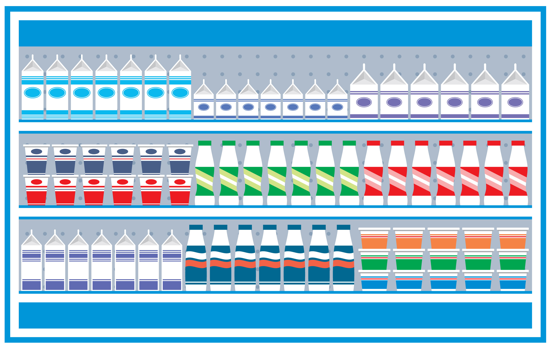
\includegraphics[width=0.6\linewidth]{Pictures/avsc.png}
%\end{figure}
%\url{https://www.kaggle.com/c/acquire-valued-shoppers-challenge}
%\end{remark}

%----------------------------------------------------------------------------------------
%   Linear optimization
%----------------------------------------------------------------------------------------

%\chapterimage{head1.png} % Chapter heading image

\chapter{Inventory Management Optimization}

Tasks of the data scientist do not only include machine learning problems but spread beyond as I mentioned in the beginning of the report. One alternative task is based on distributing, over time, a limited amount of inventory across the company stores in a retail network. Challenges specific to that environment include very short product life cycles, and store policies whereby an article is removed from display whenever one of its key sizes stocks out. 

To solve this problem it is necessary to introduce:
\begin{itemize}
\item A stochastic model predicting the sales of an article in a single store during a replenishment period
\item Determine demand forecasts, the inventory of each size initially available, and the store inventory management policy that are important for the model
\item Preform a linear optimization of the model applied to every store in the network, 
\item Compute store shipment quantities maximizing overall predicted sales, subject to inventory availability and other constraints. 

\section{Input of the optimization model}
In many clothing retail stores, an important source of negative customer experience stems from customers who have identified (perhaps after spending much time searching a crowded store) a specific article they would like to buy, but then cannot find their size on the shelf/rack. Proper management of size inventory seems even more critical to a modern retailer that offers a large number of articles produced in small series throughout the season. The presence of many articles with missing sizes would thus be particularly detrimental to the customers store experience. 
\begin{remark}
For simplicity of the discussion we will omit now the differeitiating the sizes between major (S,M,L) abd minor (XXS,XXL) and possible manager actions related to this two groups of articles. Practically the problem will also have a dynamic component because of the shipment decisions any given week. In addition the problem may involve connections between different articles that I neglect here.
\end{remark}

\section{Linearizing the problem}
A key concept for estimating the total number of sales $G$ from an initial profile of inventory will dependent now on a so-called virtual stockout time $t_s$ i.e. the time at which the store will run out of the chosen size. The primary input for the optimization model includes a demand forecast $D_i^s$ for every retail store $i$ and for every given size $s$ and the inventory avialiable in stores $I_i^s$. I also assume that all inventory is removed from customer view as soon as one of the major sizes runs out (less than four articles) at any point between succesive replenishments.

\section{Mixed Integer Problem}
The main opjective to implement an optimization model for distributing a limited amount of warehouse inventory between all stores of retailer with the goal of maximizing total expected revenue. The primary decision variables $x_i^s$ represent the shipment quantities of each size to each store. This quantities are subjected to the warehouse inventory constraint that insures the total shipment of a given size across all stores never exceed the inventory $W_s$. The secondary decision variables $z_i$ correspond to approximately expected sales across all sizes in each store $i$ for the current period under consideration. Now I can introduce a maximization problem of the sum of expected revenues in the current period.



\section{Control values}


%\begin{remark}
%Here I also omit the discussion of 
%\end{remark}



%\section{Methods}

% PULP library, 

\begin{remark}
The case of Inventory Management of a Fast-Fashion
Retail Network was studied by F. Caro and J.Gallien for the case of Zara Retail \url{https://pdfs.semanticscholar.org/80d2/4bcf23391dff0907d406cf1466d4b8aab007.pdf}. Here I base my model on their research
and write the example code for the Mixed Integer Programming \url{https://github.com/platonovserge/logistics_optimization}.
\begin{figure}[h]
\center

\includegraphics[width=0.4\linewidth]{Pictures/zara}
\end{figure}

Inventory optimization models are put in place in Zara to help the company to determine the quantity that should be delivered to every single one of its retail stores via shipments that go out twice every week. The stock delivered is strictly limited, ensuring that each store only receives just want they need. This goes towards the brand image of being exclusive while avoiding the build up of unpopular stock.
\end{remark}





\vfill
\textit{Wish you all the best, Sergey Platonov}
\end{document}